\documentclass[aip,cha,preprint,nofootinbib]{revtex4-2}

\usepackage[utf8]{inputenc}
\usepackage[T1]{fontenc}
\usepackage{amsmath,amssymb}
\usepackage{booktabs}
\usepackage{graphicx}
\graphicspath{{outputs/figures/}}
\usepackage{xcolor}
\usepackage{hyperref}
\hypersetup{colorlinks=true,linkcolor=blue!60!black,
            citecolor=blue!60!black,urlcolor=blue!60!black}

\newcommand{\Dearly}{\Delta_{\mathrm{early}}}
\newcommand{\rhoF}{\rho_F}
\newcommand{\rhoC}{\rho_C}
\newcommand{\netF}{\mathrm{net}_F}
\newcommand{\netC}{\mathrm{net}_C}
\newcommand{\Nlive}{\bar{N}_{\mathrm{live}}}
\newcommand{\Nocc}{\bar{N}^{B=8}_{\mathrm{occ}}}
\newcommand{\Gfut}{G_{\mathrm{future}}}
\newcommand{\iso}{\mathrm{iso\_emb}}
\newcommand{\fnet}{\mathrm{fine\_net}}
\newcommand{\bemp}{\beta_{\mathrm{emp}}}
\newcommand{\bdeath}{\beta_{\mathrm{death}}}
\newcommand{\blocal}{\beta_{\mathrm{local}}}
\newcommand{\bres}{\beta_{\mathrm{residual}}}

\begin{document}

\title{Observer Disagreement, Predictive Scale, and a Stable\\
       Component-Change Law in Conway's Game of Life}

\author{Kunal Bhatia}
\thanks{ORCID: \href{https://orcid.org/0009-0007-4447-6325}{0009-0007-4447-6325}}
\affiliation{Independent Researcher, Heidelberg, Germany}

\date{April 2026}

\begin{abstract}
Different coarse-grained descriptions of the same deterministic system can
yield different measured changes.
Using a component-count fine observer and an occupied-block coarse observer,
we establish three empirical regularities in Conway's Game of Life.
Early component net change predicts the full-run normalized narrative gap
between observers with partial correlation $r=-0.848$
(95\% bootstrap CI $[-0.862,-0.830]$, $N=1000$), sharpening after density
control.
The predictive scale that best forecasts a future observable depends on which
observable: time-averaged live-cell count peaks at an intermediate scale
($B=2$) while occupied-block count peaks at its own native scale ($B=8$),
with non-overlapping bootstrap confidence intervals.
A linear law linking embedded isolated cells to future component-level decline
is stable across six size-by-density conditions
(mean slope $\approx-1.52$, CV~$\approx0.09$).
Two stronger mechanism claims---global mediation through component net change,
and residual-coupling beyond death and local-neighbourhood dynamics---do not
survive their pre-specified tests.
All results are established computationally within GoL; generalisation
beyond this system remains an open empirical question.
\end{abstract}

\keywords{Conway's Game of Life, cellular automata, coarse-graining,
          observer disagreement, predictive scale, component counting,
          empirical scaling law, causal emergence}

\maketitle

\section{Introduction}
\label{sec:intro}

Different descriptions of the same dynamical system can yield different
accounts of change.
In Conway's Game of Life~\citep{gardner1970,wolfram1984}, one natural observer
counts 4-connected components of live cells---each glider is one object, each
still life is one object---while another counts occupied $8\times8$ spatial
blocks.
These are not straightforward approximations of a single underlying quantity.
Components and blocks define different effective objects, with different
characteristic lifetimes and different event statistics, and when they
disagree on whether the system underwent net creation or net destruction
over a given interval, neither is wrong.
They track different observables.

This raises three concrete questions.
First: is the disagreement between observers predictable from early dynamics
alone, before the two counts have diverged significantly?
Second: does the observation scale that best forecasts a future quantity
depend on which quantity one is forecasting?
Third: does a simple local structural count---the number of cells that are
alive but 4-disconnected from all neighbours while touching at least one
diagonal---predict future component-level change with a stable coefficient
across different system sizes and density regimes?

We answer all three affirmatively in GoL, and we also test two stronger
interpretations---that embedded isolated cells globally mediate the path from
early structure to observer disagreement, and that the slope law survives as a
positive residual over a dynamic local null---neither of which holds up.
All analyses use a single fine observer definition throughout: 4-connected
component count on the periodic torus.

\paragraph{Relation to prior work.}
\citet{hoel2013} characterise causal emergence as conditions under which a
macro-scale description carries more effective information than the micro
description; the information-integration framework from which this draws
originates with \citet{tononi1994}.
The present work is complementary but narrower, measuring the predictability
of a signed net-change difference rather than information content.
\citet{israeli2004} showed that some cellular automata admit exact
coarse-grained descriptions while others are computationally irreducible;
\citet{wolfram1984} established universality and complexity properties across
rule spaces, and \citet{langton1990} showed that GoL-like rules operate near
a phase transition supporting long-lived structured computation.
Our result is consistent with the irreducible case, in which the two
observers compute incommensurable quantities.
\citet{shalizi2003} argue that the success of coarse-graining depends on
which features of the micro-state the macro-description preserves; the
target-relative predictive structure found here is a concrete instance of
that dependence.
\citet{crutchfield1989} formalise macro-state identification through
the epsilon-machine framework, a computational-mechanics approach
complementary to the correlation-based analysis used here;
\citet{schreiber2000} operationalise cross-scale information flow through
transfer entropy.
\citet{rupe2018} identify local causal states in GoL that capture spatially
localised computational structure; the embedded isolated cells studied here
are a simpler structural class defined by connectivity rather than causal
equivalence.
\citet{vichniac1984} established cellular automata as substrates for
simulating physical systems, providing broader context for treating GoL as a
model dynamical system.
\citet{flack2017} discusses coarse-graining as a mechanism for effective
description in complex systems.

\section{Methods}
\label{sec:defs}

\subsection{Model dynamics and observers}

Let $\mathcal{G}$ be an $N\times N$ periodic grid evolving under GoL
(B3/S23) on the torus.
The \textbf{fine observer}~$F$ counts the number of 4-connected components
of live cells at each step, with periodicity enforced by breadth-first search
across opposite edges.
(\texttt{scipy.ndimage.label} operates on a flat grid and would miscount
components that span opposite edges; it is not used here.)
The \textbf{coarse observer}~$C$ counts occupied $B\times B$
non-overlapping blocks, where a block is occupied if any cell within it is
alive; default $B=8$.
We denote these counts $c^F_t$ and $c^C_t$ at step $t$.
Throughout, an observer is defined operationally as a fixed mapping from the
grid state to a scalar count.

\subsection{Derived quantities}

For a time window $[a,b]$,
\begin{align}
\netF[a,b] &= c^F_b - c^F_a, &
\netC[a,b] &= c^C_b - c^C_a, \\
\rhoF[a,b] &= \netF[a,b] / \max(c^F_a,1), &
\rhoC[a,b] &= \netC[a,b] / \max(c^C_a,1).
\end{align}
The \textbf{narrative gap} $G[a,b] = \rhoC[a,b] - \rhoF[a,b]$ is positive
when the coarse observer records more net creation and negative when the fine
observer does.
The \textbf{early imbalance} $\Dearly = \netF[0,\,t_{\rm early}]$ is the
fine-scale component net change over the first $t_{\rm early}$ steps and
serves as the predictor in Section~\ref{sec:A}.

\subsection{Cell-level structural classifier}

The mechanism tests in Section~\ref{sec:mechanism} use a classifier that
operates on individual cells, not on components.
An \textbf{embedded} cell is alive with no 4-connected live neighbours but
at least one 8-connected live neighbour.
An \textbf{alone} cell is alive with no 8-connected live neighbours.
These are cell-level structural categories; the observer variables above are
component-level and block-level counts.
The two levels are not interchangeable.

\subsection{Experimental design and statistical analysis}

We analyse three simulation ensembles; their parameters appear in
Table~\ref{tab:design}.
Each world is constructed from a per-world integer seed derived from a global
seed, so any world can be exactly regenerated from its stored seed and
density.
The predictive-scale analysis uses Ridge regression ($\alpha=1.0$) with
standardised inputs and 5-fold cross-validated $R^2$.
Decision thresholds for the primary comparisons were fixed before analysis.
No hyperparameter tuning is performed across conditions.

\begin{table}
\centering
\caption{Experimental design. Section references indicate where each
ensemble's results are reported.}
\label{tab:design}
\begin{tabular}{p{4.8cm}llllp{3cm}}
\toprule
Ensemble & Grid & $N$ & $T$ & Seed & Main statistic \\
\midrule
Observer-disagreement  & $64^2$         & 1000     & 250 & 20260325      & Pearson/partial $r$ \\
Predictive-scale       & $128^2$        & 500      & 250 & 20260326      & Ridge CV $R^2$ \\
Component-change law   & $64^2/128^2$   & 300--400 & 250 & 20260328+$k$  & OLS slope \\
\bottomrule
\end{tabular}
\end{table}

\section{Predictable Observer Disagreement}
\label{sec:A}

In a 1000-world ensemble on $64\times64$ GoL, initial densities drawn
uniformly from $[0.03,0.58]$, we measure whether $\Dearly$---the net change
in component count over the first 50 steps---predicts the full-run normalized
narrative gap $G[0,250]$.
Because initial density can drive both variables---denser worlds tend to have
more negative $\Dearly$ and more positive $G$---we compute the partial
correlation
$r(\Dearly, G\mid\rho)$, residualising both variables on initial density,
and we construct a 95\% confidence interval by bootstrapping over world rows
(1000 resamples, with the world as the resampling unit).

Table~\ref{tab:A} reports the key statistics.
The raw Pearson correlation is $r=-0.765$ ($p=1.4\times10^{-192}$).
The partial correlation is $r=-0.848$, with a 95\% bootstrap CI of
$[-0.862,-0.830]$ that excludes zero by a wide margin.
A replication on a second global seed gives partial $r=-0.835$,
confirming the result is not an artefact of the particular seed.

\begin{table}
\centering
\caption{Key statistics for the observer-disagreement analysis
($N=1000$, $64\times64$ GoL, $t_{\rm early}=50$, $B_{\rm coarse}=8$).}
\label{tab:A}
\begin{tabular}{lcc}
\toprule
Statistic & Value & \\
\midrule
$r(\Dearly, G)$                    & $-0.765$ & $p=1.4\times10^{-192}$ \\
OLS slope                          & $-1.07\times10^{-3}$
                                   & 95\% CI $[-1.12,\,-1.01]\times10^{-3}$ \\
OLS intercept                      & $0.076$ & \\
$r(\Dearly, \netC)$                & $-0.097$ & $p=0.002$ \\
Partial $r(\Dearly, G\mid\rho)$    & $-0.848$ & \\
Bootstrap 95\% CI (partial $r$)    & $[-0.862,\,-0.830]$ & world-row resampling \\
Replication (seed 20260326)        & $-0.835$ & consistent \\
\bottomrule
\end{tabular}
\end{table}

\begin{figure}
\centering
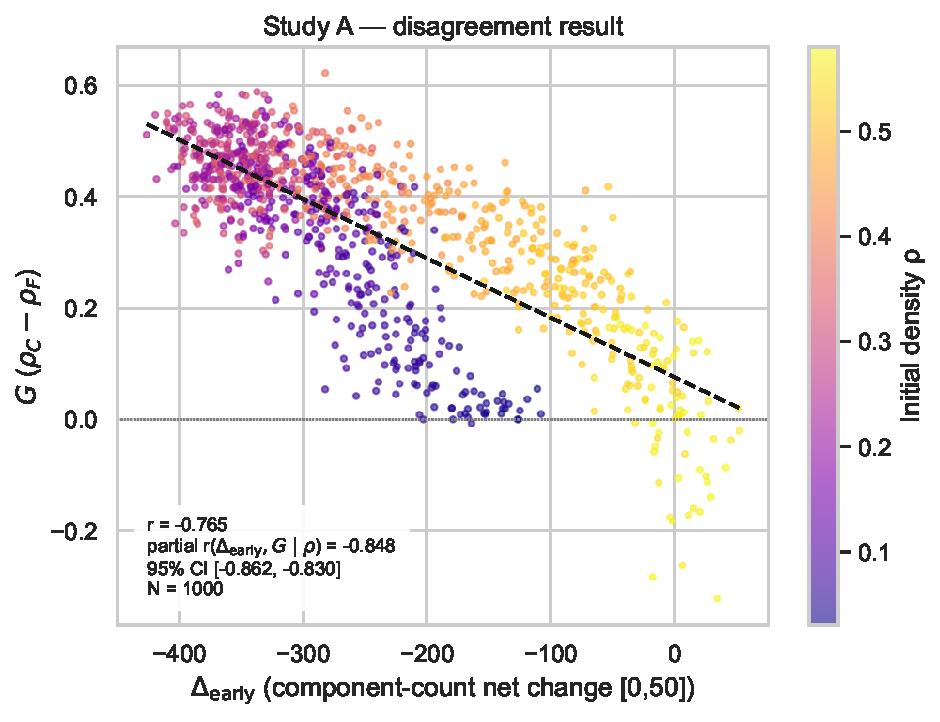
\includegraphics[width=0.82\linewidth]{fig1_studyA_scatter.pdf}
\caption{
Observer-disagreement main result.
Early fine-scale component net change $\Dearly$ predicts the full-run
narrative gap $G$.
Points are worlds coloured by initial density.
The relationship sharpens after density control:
raw $r=-0.765$, partial $r(\Dearly,G\mid\rho)=-0.848$,
95\% bootstrap CI $[-0.862,-0.830]$.
}
\label{fig:studyA_scatter}
\end{figure}

The partial correlation exceeds the raw correlation because density adds
scatter to the raw relationship.
Denser worlds have more negative $\Dearly$ and more positive $G$, so removing
the shared density channel tightens rather than loosens the association.
Within any density stratum the component net-change signal aligns more
closely with the later observer gap than the raw cross-density scatter
suggests.

The independence check $r(\Dearly, \netC)=-0.097$ ($p=0.002$) confirms that
early fine-scale dynamics carry genuine, if modest, predictive content about
coarse-scale net change over and above the density channel.
The result therefore does not reduce to a density confound.

Figure~\ref{fig:studyA_traces} shows illustrative cumulative net-change traces
for the two extreme-gap worlds: the world with the largest positive gap (fine
observer records large net destruction while the coarse observer remains near
zero) and the world with the largest negative gap (opposite pattern).
These traces are descriptive and carry no inferential weight; the
quantitative result rests on the ensemble statistics above.

\begin{figure}
\centering
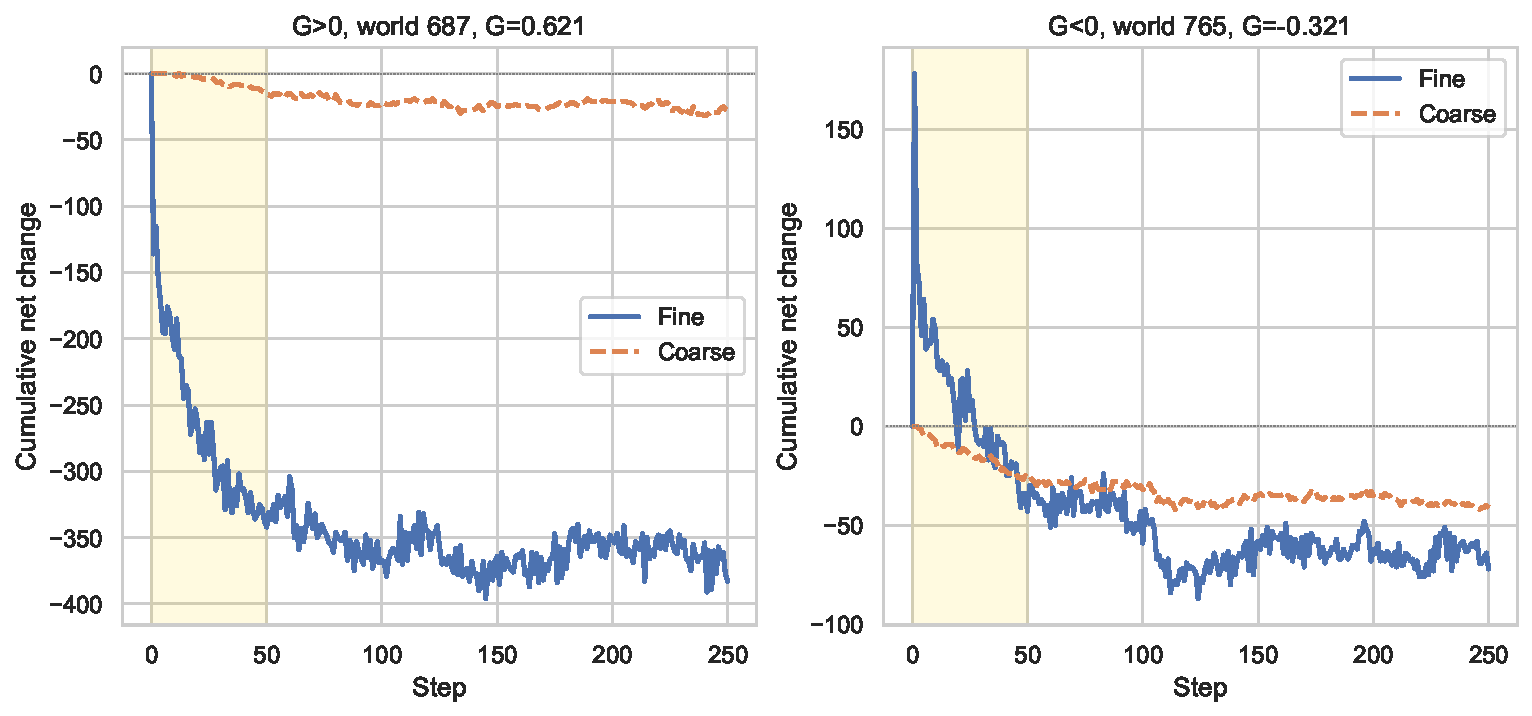
\includegraphics[width=\linewidth]{fig2_studyA_traces.pdf}
\caption{
Illustrative observer trajectories for the maximum-gap world
(left, $G=0.621$) and the minimum-gap world (right, $G=-0.321$).
These are the extreme-gap worlds selected by $\arg\max$ and $\arg\min$ of $G$,
not randomly chosen representatives.
Fine and coarse observers can accumulate opposite net-change narratives over
the same deterministic run. Yellow shading marks the early window $[0,50]$
used to compute $\Dearly$.
These panels are descriptive only and are not used in the inferential test.
}
\label{fig:studyA_traces}
\end{figure}

\section{Predictive Scale is Target-Relative}
\label{sec:B}

\subsection{Setup}

In a 500-world $128\times128$ ensemble, density uniform on $[0.20,0.35]$,
we test whether the observation scale that best predicts a future observable
depends on which observable one chooses.
The question has a direct scientific meaning: if there is a single
universally optimal scale for prediction, then scale choice affects only
precision, not structure.
If different future quantities prefer different scales, the implication is
stronger: the choice of scale is not merely a resolution question but a
question about which aspects of the post-transient state are relevant to
which aspects of the future.

Features are extracted at five scales $B\in\{1,2,4,8,16\}$, where at $B=1$
the feature time series uses BFS component counts (the fine observer defined
above) and at $B>1$ it uses occupied-block counts.
The predictor window is $[50,100]$; the target window is $[100,200]$.
The two \textbf{primary targets} are $\Nlive$ (time-averaged live-cell count)
and $\Nocc$ (time-averaged occupied-$B=8$-block count).
Two \textbf{secondary targets} are $\bar{A}$ (mean step-to-step absolute
change in live cells) and $\Gfut$ (narrative gap $G[100,200]$);
secondary targets are reported but do not gate the main conclusion.
The comparison varies the scale at which predictor features are extracted,
while the target definitions themselves remain fixed.

Before analysis, we specified that evidence for target-relative predictive
scale would require non-overlapping bootstrap peak-$B$ intervals for at least
two primary targets, with one peak at $B\leq2$ and another at $B\geq4$.
The negative controls are static IC features and early-transient $[0,50]$
features, expected to yield no positive held-out $R^2$ for primary targets.

\subsection{The negative controls are clean}

Of the 20 primary-target static-or-early conditions, none exceeds $R^2=0.04$.
This establishes that the predictive signal is not inherited from the initial
condition or from the statistics of the early die-off.
The information that forecasts the future emerges only after the initial
transient has settled and the surviving spatial structure has largely
stabilised.
In a deterministic system the initial condition fully specifies all future
states, but low-dimensional statistical summaries of that initial
condition---at any scale---cannot access the relevant degrees of freedom
for forecasting.

\begin{figure}
\centering
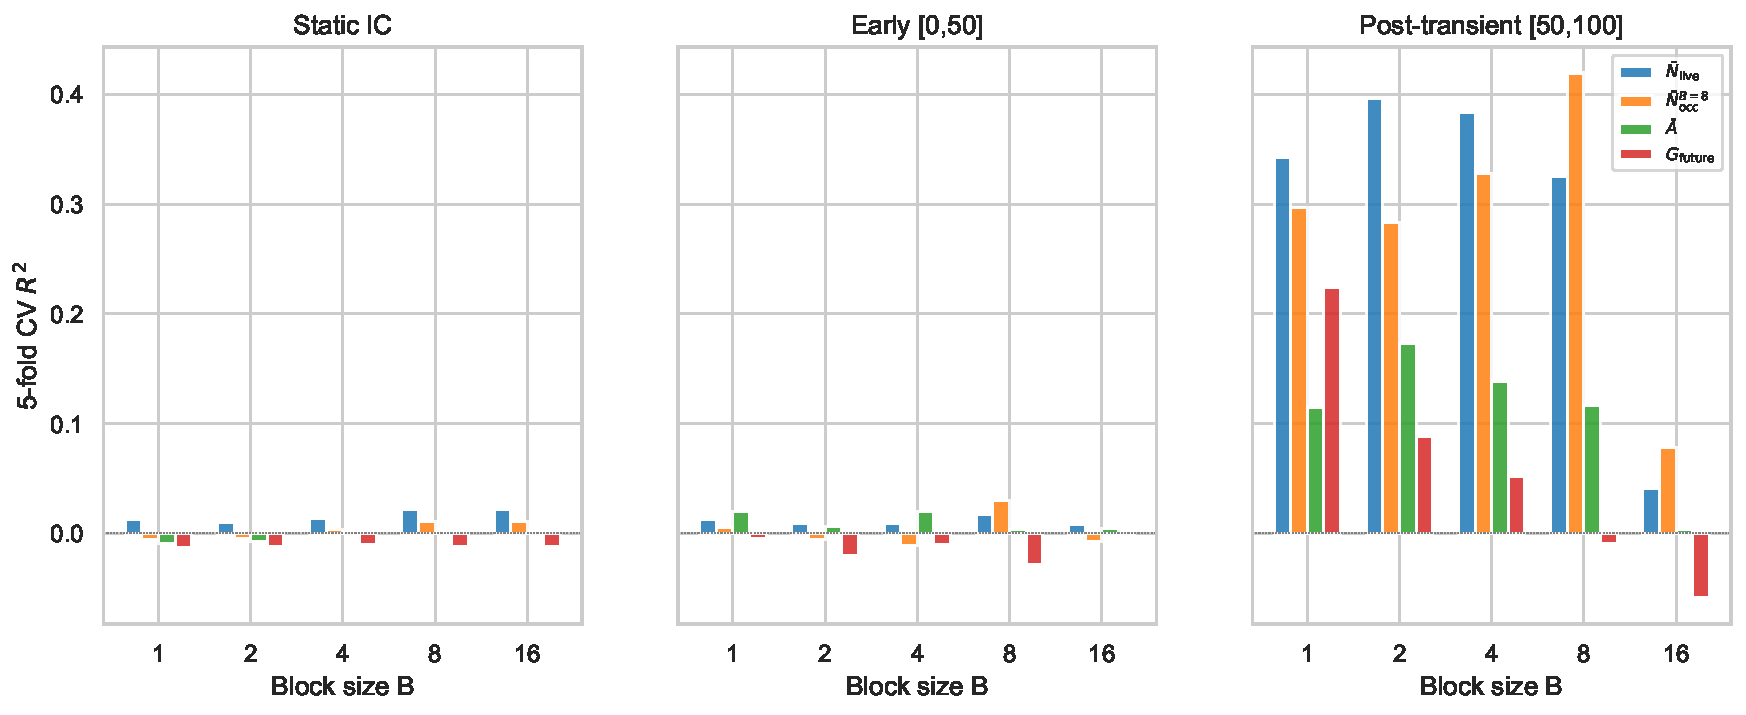
\includegraphics[width=\linewidth]{fig3_studyB_windows.pdf}
\caption{
Predictive signal across temporal windows.
Static initial-condition features and early-transient features remain weak for
the primary targets, while post-transient features carry substantial predictive
power. This shows the clean negative-control result.
}
\label{fig:studyB_windows}
\end{figure}

\subsection{Post-transient predictive structure}

The post-transient window contains the predictive signal.
For the primary targets, $\Nlive$ reaches cross-validated
$R^2=0.396$ at $B=2$, while $\Nocc$ reaches $R^2=0.420$ at $B=8$
(Table~\ref{tab:B_r2}).
The negative-control audit is clean: 0/20 primary-target static-or-early
conditions exceed $R^2=0.04$.
This rules out the possibility that the result is a trivial echo of the
initial condition or of the earliest transient.

\begin{table}
\centering
\caption{Post-transient $[50,100]\to[100,200]$ cross-validated $R^2$ by
target and observation scale. Bold entries mark the peak scale per primary
target.}
\label{tab:B_r2}
\begin{tabular}{l ccccc}
\toprule
Target & $B=1$ & $B=2$ & $B=4$ & $B=8$ & $B=16$ \\
\midrule
$\Nlive$ (primary)    & 0.343 & \textbf{0.396} & 0.383 & 0.325 & 0.041 \\
$\Nocc$ (primary)     & 0.297 & 0.283 & 0.328 & \textbf{0.420} & 0.078 \\
\midrule
$\bar{A}$ (secondary) & 0.115 & 0.173 & 0.139 & 0.116 & 0.003 \\
$\Gfut$ (secondary)   & 0.224 & 0.088 & 0.052 & $-0.009$ & $-0.059$ \\
\bottomrule
\end{tabular}
\end{table}

\begin{figure}
\centering
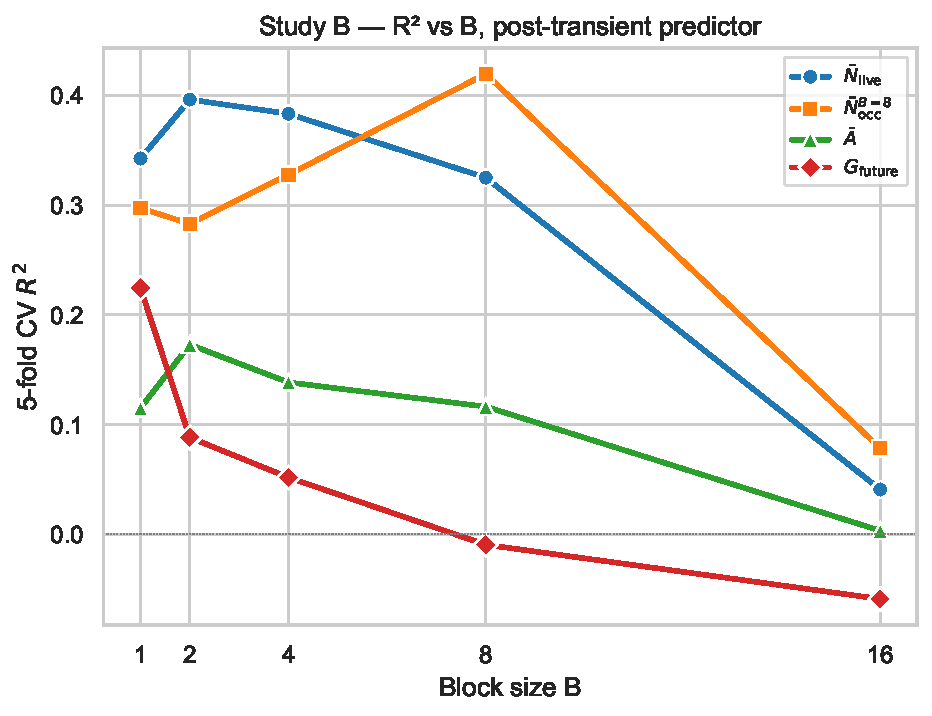
\includegraphics[width=0.82\linewidth]{fig4_studyB_r2_vs_B.pdf}
\caption{
Target-relative predictive scales.
Future live-cell count peaks at $B=2$, while future occupied-block count peaks
at $B=8$. The two primary targets prefer different observation scales within
the same deterministic system.
}
\label{fig:studyB_r2}
\end{figure}

Table~\ref{tab:B_peaks} gives the bootstrap peak-$B$ analysis.
The confidence interval for $\Nlive$ is $[2,4]$; the interval for $\Nocc$
is $[8,8]$---meaning not one of the 1000 bootstrap draws placed the peak
anywhere other than $B=8$.
The two intervals do not overlap, and the required pattern (one peak at
$B\leq2$, another at $B\geq4$) is present.

\begin{table}
\centering
\caption{Bootstrap peak-$B$ confidence intervals for primary targets
(1000 resamples, world-row resampling).}
\label{tab:B_peaks}
\begin{tabular}{lcc}
\toprule
Target & Point peak $B$ & 95\% CI \\
\midrule
$\Nlive$ & 2 & $[2,\;4]$ \\
$\Nocc$  & 8 & $[8,\;8]$ \\
\midrule
CI overlap & \multicolumn{2}{c}{None} \\
Required pattern ($B\leq2$ and $B\geq4$ among primaries) & \multicolumn{2}{c}{Present} \\
\midrule
Negative control: primary-target static/early with $R^2>0.04$ & \multicolumn{2}{c}{0/20} \\
\bottomrule
\end{tabular}
\end{table}
\noindent\textit{Note on negative controls.}
At $\rho\in[0.20,0.35]$ on a $128^2$ grid, $B=16$ blocks cover 256 cells
each; virtually all blocks are occupied, so $B=16$ static features are
near-constant across worlds and their $R^2\approx0$ trivially.
The 4 conditions involving $B=16$ static features are therefore degenerate.
Excluding them, 0/16 non-trivial negative controls exceed the threshold.

\subsection{Interpretation}

This provides direct evidence, within this system, against the existence of
a single privileged predictive scale.
The scale preferences have a qualitative logic.
$\Nlive$ benefits from a smoothing scale ($B=2$) that attenuates
single-component fluctuations while preserving the spatial heterogeneity of
surviving structures; neither the finest scale nor the coarse-block scale
achieves this trade-off as well.
$\Nocc$ is best predicted at its own native scale ($B=8$): the coarse
observer's own dynamics are maximally informative about its own future
population, a form of internal self-consistency that does not generalise to
other observables.
The secondary target $\Gfut$ peaks at $B=1$, consistent with
Section~\ref{sec:A}: the observer gap is driven by fine-scale events
invisible to coarser descriptions.
These are different questions about the same deterministic system, and they
are best answered from different vantage points.

The two primary targets' bootstrap peak-$B$ confidence intervals do not
overlap: $\Nlive$ peaks at $B=2$ with CI $[2,4]$, while $\Nocc$ peaks at
$B=8$ with CI $[8,8]$.
The exact $[8,8]$ interval for $\Nocc$ is especially strong: in the bootstrap
resampling, no alternative scale displaced the block observer's own native
scale as the best predictor of its future occupied-block population.

\section{A Stable Law for Component Change}
\label{sec:D}

\subsection{Motivation for the embedded-isolated-cell predictor}

In the post-transient GoL regime, the grid contains a mixture of stable
structures---still lifes, oscillators, and occasional gliders---interspersed
with near-isolated cells that are alive but structurally marginal.
An embedded cell is alive, has no 4-connected live neighbours (so it is not
part of any larger component), but does have at least one diagonal live
neighbour.
This structural configuration makes such cells natural candidates as
predictors.
The analysis below tests whether their count at the start of a measurement
window statistically predicts how much the component count will change over
that window.

\subsection{Design and criterion}

The analysis covers six conditions:
GoL on $64^2$ and $128^2$ grids, each at low ($\rho\in[0.10,0.20]$),
mid ($[0.25,0.35]$), and high ($[0.35,0.50]$) density bands, one fixed seed
per condition.
In each condition we fit
\begin{equation}
\label{eq:ols}
\fnet \;\sim\; \bemp\cdot\iso + c(\text{area})
\end{equation}
by OLS, where $\fnet = \netF[T_0,T_1]$ and $\iso$ is the embedded isolated
cell count at $T_0$.
The criterion, specified in advance, is CV$(\bemp)\leq0.20$ across the six
conditions.

\subsection{Results}

Table~\ref{tab:D} reports the slope estimates.

\begin{table}
\centering
\caption{OLS slope estimates across the six GoL conditions.
The CV across conditions is well below the threshold of 0.20.}
\label{tab:D}
\begin{tabular}{lccc}
\toprule
Condition & $\bemp$ & $R^2$ & \\
\midrule
$64^2$, low density   & $-1.462$ & 0.413 & \\
$64^2$, mid density   & $-1.613$ & 0.338 & \\
$64^2$, high density  & $-1.383$ & 0.296 & \\
$128^2$, low density  & $-1.767$ & 0.684 & \\
$128^2$, mid density  & $-1.404$ & 0.302 & \\
$128^2$, high density & $-1.498$ & 0.328 & \\
\midrule
Mean $\pm$ SD & $-1.521 \pm 0.133$ & & \\
CV            & $0.087$ & & \\
\bottomrule
\end{tabular}
\end{table}

\begin{figure}
\centering
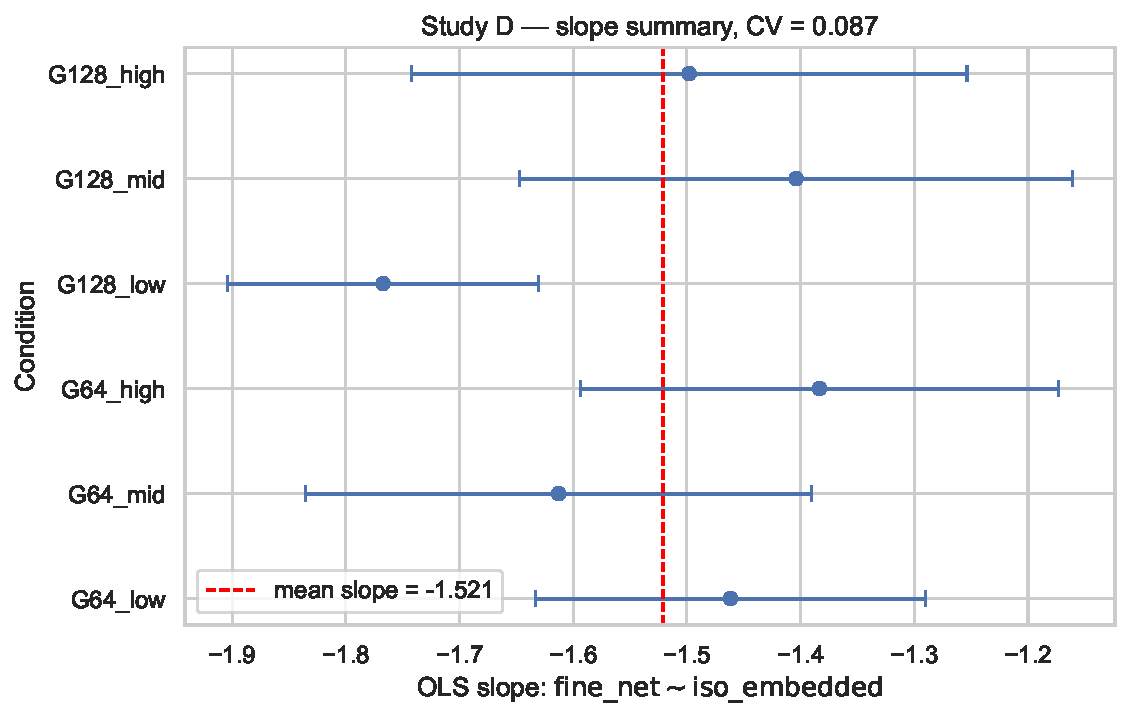
\includegraphics[width=0.82\linewidth]{fig6_studyD_slope_summary.pdf}
\caption{
Slope estimates across the six GoL conditions.
Points show OLS slopes and horizontal bars show 95\% confidence intervals.
The mean slope is approximately $-1.52$ and the cross-condition coefficient of
variation is $0.087$, below the pre-specified stability threshold.
}
\label{fig:studyD_slopes}
\end{figure}

The slope varies between $-1.38$ and $-1.77$ across grid sizes and density
regimes.
The mean slope is $-1.52$, with a standard deviation of $0.13$ and
CV~$=~0.087$.
This is well below the threshold, establishing
\begin{equation}
\label{eq:law}
\fnet \;\approx\; -1.52\cdot\iso + c(\text{area})
\qquad\text{CV}=0.087,\quad\text{six GoL conditions}
\end{equation}
as a stable empirical law across these conditions.
Under the component-count fine observer used throughout this paper, the mean
slope is approximately $-1.52$ units of future component net change per
embedded isolated cell.

\subsection{Interpretation}

The law is empirical, not mechanistic.
It says that embedded isolated cells predict future component-level decline
with a coefficient stable across size and density.
It does not say why, and Section~\ref{sec:mechanism} will show that the
simplest mechanistic account---that the law is driven by a positive residual
coupling over and above trivial null dynamics---is not supported.
The distinction matters: the law is as solid as the CV figure suggests; the
mechanism behind it is an open question.

The $R^2$ values vary more than the slopes do, ranging from 0.30 to 0.68.
This variation reflects the different dynamical character of the density
regimes rather than instability in the relationship: in low-density
conditions the future trajectory is more structured and thus easier to
predict from a single feature, while in high-density conditions the
dynamics are more variable.

\subsection{Circularity and selection concerns}

An obvious concern is circularity: a predictor can appear powerful if it is
defined using the very future behaviour it is later said to predict.
Our construction avoids this.
Embedded isolated cells are identified entirely from the configuration at the
observation time~$T_0$, using a contemporaneous structural criterion
(Section~\ref{sec:defs}): alive, no 4-connected live neighbours, at least one
diagonal live neighbour.
The outcome variable~$\fnet$---net fine-scale component change over the
subsequent window---is measured afterward and plays no role in the object
definition.
The relation is therefore temporally prospective, not definitional.

A second concern is that the predictor might re-express current fragmentation,
making the law a bookkeeping identity rather than a predictive regularity.
But the target is future change in component count, not the present count
itself, and the empirical slope is a cross-condition regularity whose
stability (CV~$=0.087$) would not be expected from an accounting tautology.
The mediation and null-decomposition analyses in Section~\ref{sec:mechanism}
further confirm that the relationship carries non-trivial structure.

A third concern is selection: were many candidate predictors tried, with only
the successful one reported?
The embedded isolated cell is the structurally motivated candidate---it is the
only cell-level class that is simultaneously 4-disconnected (hence a singleton
component) and 8-connected to an existing structure (hence embedded rather than
truly alone).
No automated search over predictor families was conducted; the comparison
reported in Section~\ref{sec:mechanism} between embedded and alone cells is
the only competitor tested and is presented in full.

\section{Tests of Stronger Mechanism Interpretations}
\label{sec:mechanism}

The preceding sections establish three empirical regularities.
This section tests two stronger mechanism interpretations: first, whether
embedded isolated cells mediate the path from early structure to observer
disagreement; second, whether the empirical law survives as a positive excess
beyond death and local-neighbourhood nulls.
Neither interpretation is supported by the present analyses.

\subsection{Global mediation}

The proposed mechanism is that early accumulation of embedded isolated cells
drives future component net change, which in turn drives the narrative gap.
We test this by the product-of-coefficients method, controlling for density
in both the mediator and outcome regressions, with a 95\% CI from 1000
bootstrap resamples.

Embedded count predicts $G$ more strongly than alone count
($r=0.471$, partial $r=0.632$ vs.\ $r=0.328$, partial $r=0.403$),
and embedded count strongly predicts $\fnet$
($r=-0.731$, partial $r=-0.608$).
These comparisons show that embedded isolated cells are the stronger
discriminator.

\begin{figure}
\centering
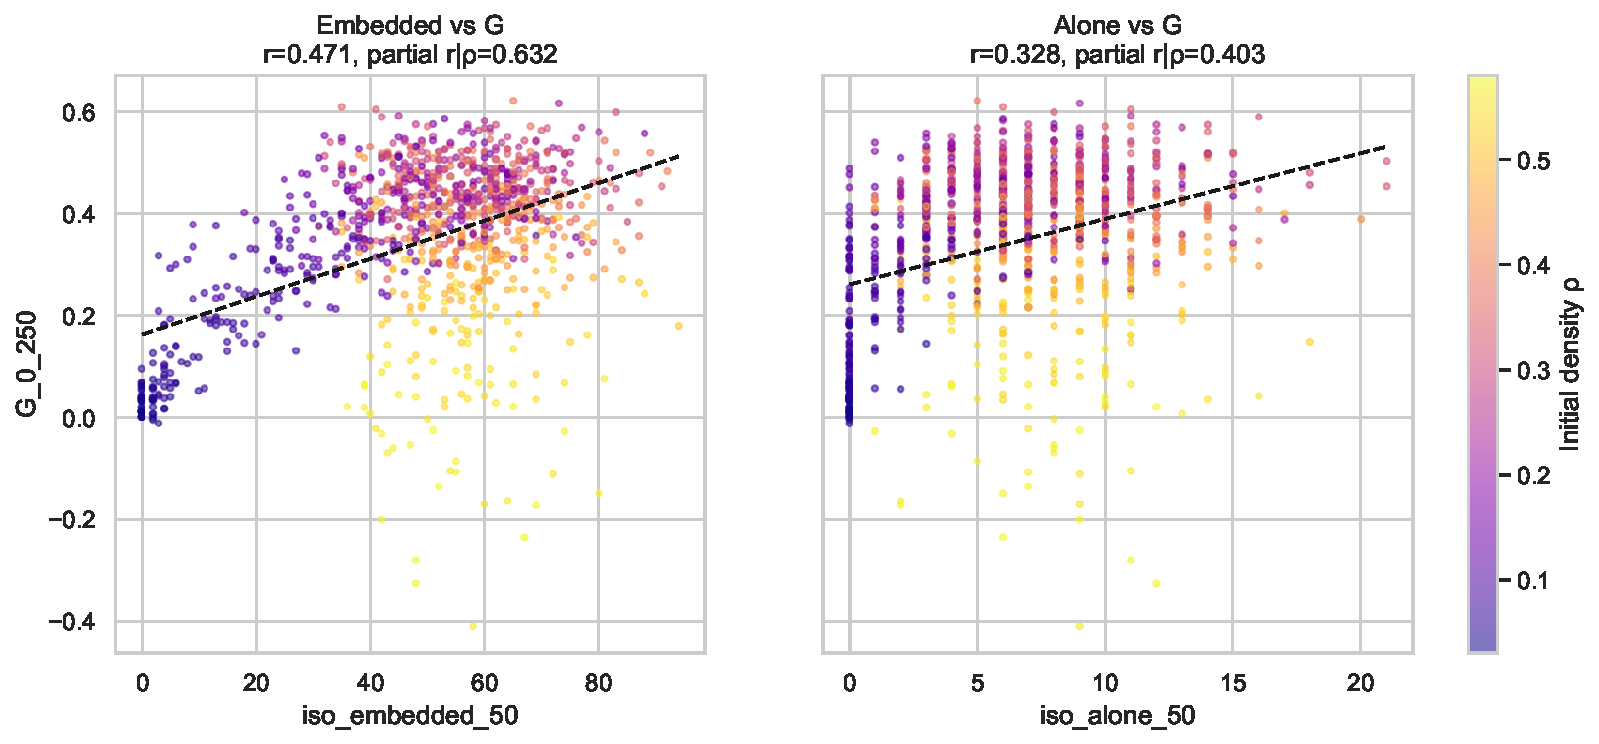
\includegraphics[width=\linewidth]{fig5_studyC_embedded_vs_alone.pdf}
\caption{Association between isolated cell count at $t=50$ and narrative gap
$G$ for embedded cells (left) and alone cells (right).
Embedded cells are the stronger discriminator ($r=0.471$, partial $r=0.632$
vs $r=0.328$, partial $r=0.403$ for alone cells).
The mediation test asks whether this association runs through future component
net change; it does not meet the pre-specified threshold.}
\label{fig:C_discriminator}
\end{figure}

However, the mediation test fails.
The estimated indirect effect is $-4.61\times10^{-4}$, with mediation fraction
$-0.072$ and bootstrap 95\% CI $[-0.145,\,-0.007]$.
This interval lies entirely below zero and fails to exceed $0.50$.
The supported reading is therefore that embedded isolated cells are
harbingers of later disagreement, not established global mediators of it.

A design note: the outcome $G$ is computed over the full $[0,250]$ window
while the mediator $\fnet$ uses the post-predictor window $[50,250]$.
The mismatch means $G$ absorbs dynamics from steps $0$--$50$ that precede the
predictor measurement, which can only attenuate the mediation estimate.
A fully aligned test would use $G_{[50,250]}$ as the outcome; we do not
re-run it here because the mediation fraction already fails by a wide margin
($-0.072$ with CI entirely below zero).

\subsection{Null decomposition of the component-change law}

We decompose $\bemp = \bdeath + \blocal + \bres$ and ask whether $\bres$
represents a positive excess beyond trivial null dynamics.
The death term $\bdeath=-1.0$ is analytically fixed: each embedded cell that
dies removes exactly one component.
In practice, roughly 35--41\% of embedded cells die across the six conditions
(empirical survival probability 0.59--0.66); the decomposition is a formal
accounting identity, not a prediction based on the actual death rate.
A static local null (no neighbourhood context) gives $\blocal\approx0$,
leaving $\bres\approx\bemp-\bdeath$; the excess index
$\chi=\bres/|\bdeath+\blocal|$ is negative in all six conditions
($\chi\in[-0.77,-0.38]$), so even under the static null the residual is not
positive.

A dynamic local null, using $5\times5$ neighbourhood patches centred on
each focal cell, gives $\blocal\in[0.35,0.51]$ across conditions.
Here $\blocal$ is an accounting term defined from mean single-step local
structural contributions, not a regression coefficient from a separate
null-model fit.
Local neighbourhood context is itself predictive and non-negligible.
Under this null, $\bres\in[-1.12,-0.81]$ and $\chi_{\rm mean}=-1.78$; no
condition satisfies $\chi\geq0.25$.
The residual remains large and negative: not a small positive excess over
local dynamics, but a large negative residual after subtracting the death
and local terms.

\begin{figure}
\centering
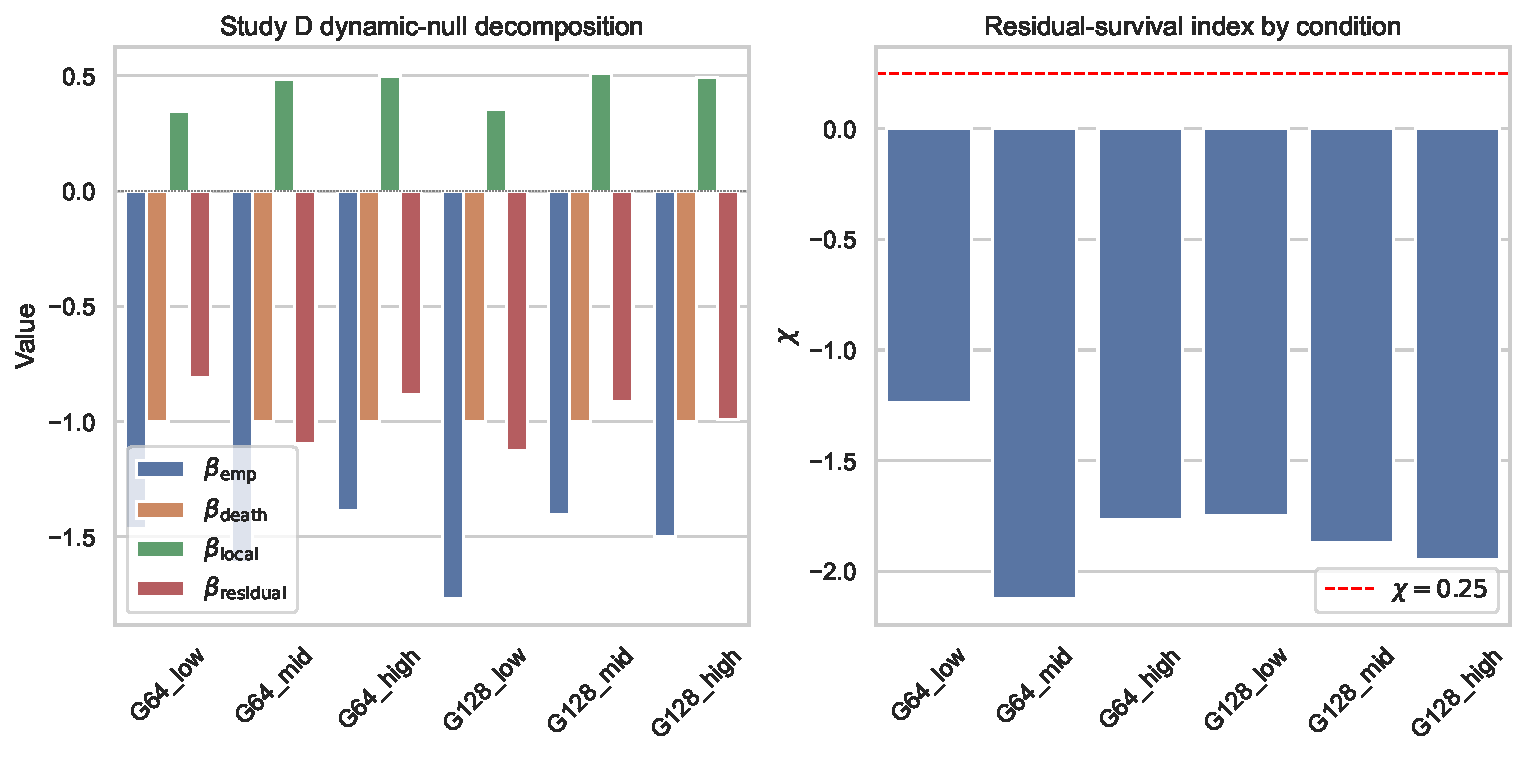
\includegraphics[width=\linewidth]{fig7_studyD_decomposition.pdf}
\caption{
Dynamic-null decomposition of the component-change law.
Across conditions, the empirical slope is stable, but the residual term does
not survive as a positive excess beyond death and local-neighbourhood
contributions. The empirical law is therefore supported; the stronger
residual-coupling interpretation is not.
}
\label{fig:studyD_decomposition}
\end{figure}

The empirical law is stable (CV~$=~0.087$).
The claim that it arises from a positive residual coupling beyond death and
local neighbourhood dynamics is not supported.

\section{Discussion}
\label{sec:disc}

\paragraph{Supported results.}
Three empirical regularities in GoL are robust to fixed observer definitions
and fixed decision thresholds.
Observer disagreement is strongly predictable from early fine-scale component
dynamics: the partial correlation between early component net change and the
full-run narrative gap is $r=-0.848$ and sharpens after density control.
The scale that best forecasts a future quantity depends on which quantity:
future live-cell count peaks at $B=2$, future occupied-block count peaks at
$B=8$, and the two bootstrap confidence intervals do not overlap.
The embedded-isolate slope is stable across six size-by-density conditions
with CV~$=0.087$.
Together these results show that the choice of coarse-grained description
in GoL is not arbitrary: different measurement schemes yield different but
lawful summaries of change, and their disagreement is itself predictable from
early local structure.

\paragraph{Unsupported mechanism interpretations.}
Two mechanism interpretations are not supported.
Embedded isolated cells are harbingers of later observer disagreement, but
not established global mediators of it: the product-of-coefficients mediation
fraction is $-0.072$ with CI entirely below zero.
The empirical slope law does not emerge as a positive residual over the
dynamic local null: $\chi < 0$ in all six conditions.
The empirical structure is well-characterised; the mechanistic account is not
yet in hand.

Follow-up audits have probed the mechanism directly across four approaches.
(i)~Exact one-cell deletion: the per-cell causal effect recovers only part of
the raw slope.
(ii)~$k$-delete ladder: per-cell effects decrease with $k$, ruling out
collective additivity as a rescue.
(iii)~Controlled-carrier regression: pooled residual signal is weak and
within-condition stability is not recovered.
(iv)~Refined local carrier ($d_2$-adjacency): does not improve slope
stability and worsens it in several conditions.
None of the tested local accounts rescues a per-cell causal reading.
The slope is best treated as a stable empirical structural relation:
$\iso$ is the best simple carrier of the raw law, but the law does not reduce
to a direct per-cell causal rate.

\paragraph{On the null decomposition baseline.}
The choice $\bdeath=-1.0$ is analytically exact rather than empirically
estimated: an embedded cell is a 4-connected singleton component, so its
death must reduce the component count by exactly one.
An alternative would scale $\bdeath$ by the actual death fraction
($\approx0.37$), giving $\bdeath\approx-0.37$ and shifting $\bres$ toward
zero.
We retain $-1.0$ because it is the maximum individual-cell contribution,
making $\bres$ a conservative lower bound on any excess coupling: a negative
$\bres$ even under this upper-bound baseline rules out the positive-coupling
story more forcefully than a scaled baseline would.
The large negative $\bres$ ($\chi_{\rm mean}=-1.78$) therefore cannot be
explained away by the choice of baseline; any reasonable rescaling leaves the
qualitative conclusion intact.

\paragraph{Observer definition and numerical scope.}
All analyses in this paper use a single fine measurement scheme:
4-connected component count on the torus.
The predictor---embedded isolated cell count---is defined from present-time
structure only and does not use future trajectory information; the law is
prospective, not circular (Section~\ref{sec:D}).
Under this scheme the mean slope is approximately $-1.52$ units of future
component net change per embedded isolated cell.
The slope is design-dependent: a narrower-scope study restricted to
$\rho\in[0.20,0.35]$ with a 100-step future window yields
$\beta\approx-1.27$ with lower variance (CV~$=0.063$).
The sign and order of magnitude are stable across tested designs; the
functional dependence $\beta(\rho,K,\text{rule set})$ is uncharacterised.
Because component counts and live-cell counts behave differently, this
coefficient should not be compared directly to live-cell-based estimates.

\paragraph{Open problems.}
The mechanism question is the central open problem.
The global mediation path through $\fnet$ is insufficient, and the four
follow-up audits described above have closed the local per-cell causal
reading.
The leading open question is whether $\iso$ functions as a compact marker of
a \textit{world-level fragility regime}---a global structural property of
the grid state---rather than as the mechanistic atom whose individual deaths
drive the slope.
Under a fragility-field interpretation, worlds with more embedded cells are
in a structural regime where component-level decline is collectively favoured;
the law would hold at the population level not because each cell individually
contributes $-1.52$ components, but because the count indexes broader
grid-level vulnerability.
This interpretation is consistent with the finding that
$\iso$-targeted deletion performs \emph{worse than random} across 12/12
size-by-density conditions in a matched-budget deletion study, while
coarse block-targeted deletion outperforms $\iso$-targeted in all 12
conditions---an anti-alignment between predictive-best sites and
causally effective sites that is expected if the count is a regime marker
rather than a causal lever.

A temporal robustness check (temporal stride $m\in\{1,2,4\}$) confirms the
slope law is sign-consistent at all tested strides, with a two-phase $R^2$
degradation pattern: $R^2$ drops approximately 25--30\% from $m=1$ to
$m=2$, then stabilises from $m=2$ to $m=4$.
The law is not locked to the finest temporal articulation tested; the null
decomposition at $m>1$ is deferred.

Generalisation beyond GoL is an open empirical question.
Among Life-like rules, HighLife (B36/S23) is a natural first candidate:
it supports a richer replicator ecology, which would test whether the
embedded-cell predictor remains valid when more complex persistent structures
dominate the post-transient regime.
Day~\&~Night (B3678/S34678), which has a symmetric birth/death rule, would
separate the effects of rule asymmetry from the structural mechanism.
Rules near the computational phase transition---at Langton's $\lambda\approx0.273$---
would test whether the observer disagreement and the slope law are specific to
GoL's particular order/chaos boundary or persist across the rule-space continuum.
The functional dependence $\beta(\rho,K,\text{rule set})$ is fully uncharacterised
and is the most direct route to understanding the scope of the empirical law.

\begin{acknowledgments}
No external funding was received for this work. The author has no conflicts
of interest to declare. Simulations were performed using Python~3 with
NumPy, SciPy, scikit-learn, pandas, Matplotlib, and seaborn.
\end{acknowledgments}

\section*{Data and Code Availability}

All code, simulation outputs, and figure sources are available at
\url{https://github.com/kunalb541/CA}.

\begin{thebibliography}{99}

\bibitem[Crutchfield and Young(1989)]{crutchfield1989}
Crutchfield, J.\,P.\ and Young, K.\ (1989).
Inferring statistical complexity.
\textit{Physical Review Letters}, 63(2):105--108.

\bibitem[Flack(2017)]{flack2017}
Flack, J.\,C.\ (2017).
Coarse-graining as a downward causation mechanism.
\textit{Phil.\ Trans.\ R.\ Soc.\ A}, 375(2109):20160338.

\bibitem[Gardner(1970)]{gardner1970}
Gardner, M.\ (1970).
Mathematical games: The fantastic combinations of John Conway's new
solitaire game ``life''.
\textit{Scientific American}, 223(4):120--123.

\bibitem[Hoel et al.(2013)]{hoel2013}
Hoel, E.\,P., Albantakis, L., and Tononi, G.\ (2013).
Quantifying causal emergence shows that macro can beat micro.
\textit{Proc.\ Natl.\ Acad.\ Sci.}, 110(49):19790--19795.

\bibitem[Israeli and Goldenfeld(2004)]{israeli2004}
Israeli, N.\ and Goldenfeld, N.\ (2004).
Computational irreducibility and the predictability of complex physical
systems.
\textit{Phys.\ Rev.\ Lett.}, 92(7):074105.

\bibitem[Langton(1990)]{langton1990}
Langton, C.\,G.\ (1990).
Computation at the edge of chaos: Phase transitions and emergent computation.
\textit{Physica D: Nonlinear Phenomena}, 42(1--3):12--37.

\bibitem[Rupe and Crutchfield(2018)]{rupe2018}
Rupe, A.\ and Crutchfield, J.\,P.\ (2018).
Local causal states and discrete coherent structures.
\textit{Chaos}, 28(7):075312.

\bibitem[Schreiber(2000)]{schreiber2000}
Schreiber, T.\ (2000).
Measuring information transfer.
\textit{Physical Review Letters}, 85(2):461--464.

\bibitem[Shalizi and Moore(2003)]{shalizi2003}
Shalizi, C.\,R.\ and Moore, C.\ (2003).
What is a macrostate? Subjective observations and objective dynamics.
\textit{arXiv preprint cond-mat/0303625}.

\bibitem[Tononi et al.(1994)]{tononi1994}
Tononi, G., Sporns, O., and Edelman, G.\,M.\ (1994).
A measure for brain complexity: Relating functional segregation and
integration in the nervous system.
\textit{Proc.\ Natl.\ Acad.\ Sci.}, 91(11):5033--5037.

\bibitem[Vichniac(1984)]{vichniac1984}
Vichniac, G.\,Y.\ (1984).
Simulating physics with cellular automata.
\textit{Physica D: Nonlinear Phenomena}, 10(1--2):96--116.

\bibitem[Wolfram(1984)]{wolfram1984}
Wolfram, S.\ (1984).
Universality and complexity in cellular automata.
\textit{Physica D: Nonlinear Phenomena}, 10(1--2):1--35.

\end{thebibliography}

\end{document}
